\documentclass[a4paper,12pt]{report} % добавить leqno в [] для нумерации слева

%%% Работа с русским языком
\usepackage{cmap}					% поиск в PDF
\usepackage{mathtext} 				% русские буквы в формулах
\usepackage[T2A]{fontenc}			% кодировка
\usepackage[utf8]{inputenc}			% кодировка исходного текста
\usepackage[english,russian]{babel}	% локализация и переносы

%%% Дополнительная работа с математикой
\usepackage{amsmath,amsfonts,amssymb,amsthm,mathtools} % AMS
\usepackage{icomma} % "Умная" запятая: $0,2$ --- число, $0, 2$ --- перечисление

%% Номера формул
\mathtoolsset{showonlyrefs=true} % Показывать номера только у тех формул, на которые есть \eqref{} в тексте.

%% Шрифты
\usepackage{euscript}	 % Шрифт Евклид
\usepackage{mathrsfs} % Красивый матшрифт

%% Свои команды
\DeclareMathOperator{\sgn}{\mathop{sgn}}

%\setlength\parindent{0ex}
%\setlength\parskip{0.3cm}

%%% Заголовок
\author{Волков Павел А-14-19}
\title{Типовой расчет №12 по численным методам Вариант 3}
\date{\today}

\usepackage{graphicx}

\begin{document} % конец преамбулы, начало документа

\maketitle

\newpage
\section*{Задание}

Выполнить три итерации по методу Зейделя для системы уравнений $Ax = b$(не переставляя строк). В качастве начального приближения взять нулевой вектор. Изобразить графически поведение итерационного процесса. Сопоставить наблюдаемое поведение метода с выполнением достаточных условий сходимости метода.

\begin{gather*}
	A = 
	\begin{pmatrix}
		4 & 3 \\
		4 & 4 \\
	\end{pmatrix}, b = 
	\begin{pmatrix}
		12 \\ 12
	\end{pmatrix}
\end{gather*}

\section*{Решение}

Нетрудно заметить, что точным решением является вектор $(3, 0)^T$. Построим итерационный процесс по методу Зейделя:

\[
	\left\{
		\begin{aligned}
		x_1^{(n+1)} = -0.75x_2^{(n)} + 3  \\
		x_2^{(n+1)} = -x_1^{(n+1)} + 3 \\
		\end{aligned}
	\right.
\]

\[
	x^{(0)} = 
	\begin{pmatrix}
		0 \\ 0
	\end{pmatrix},
	x^{(1)} = 
	\begin{pmatrix}
		3 \\ 0
	\end{pmatrix},
	x^{(2)} = 
	\begin{pmatrix}
		3 \\ 0
	\end{pmatrix},
	x^{(3)} = 
	\begin{pmatrix}
		3 \\ 0
	\end{pmatrix},
\]

Геометрическая интерпретация метода:

\noindent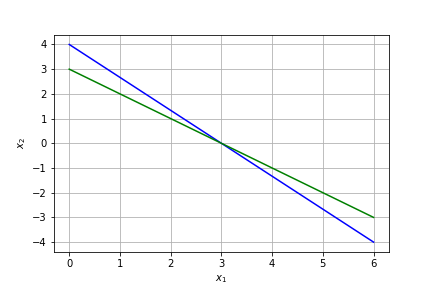
\includegraphics[height=8cm]{regular_calc_12.png}

Проверка условий сходимости:

\begin{gather*}
	B = 
	\begin{pmatrix}
		0 & -3/4 \\
		-1 & 0
	\end{pmatrix},
	B_1 =
	\begin{pmatrix}
		0 & 0 \\
		-1 & 0
	\end{pmatrix},
	B_2 = 
	\begin{pmatrix}
		0 & -3/4 \\
		0 & 0
	\end{pmatrix} \\
	||B_1|| + ||B_2|| = 5/4 > 1
\end{gather*}

Критерий $||x^{(n)} - x^{(n-1)}|| < \dfrac{1 - ||B||}{||B_2||} \varepsilon$ не работает.

Воспользуемся другим критерием:

\begin{gather*}
	r^{(0)} = Ax^{(0)} - b = \begin{pmatrix} -12 \\ -12 \end{pmatrix}, ||r^{(0)}||_{\infty} = 12 \\
	r^{(1)} = Ax^{(1)} - b = \begin{pmatrix} 0 \\ 0 \end{pmatrix}, ||r^{(1)}||_{\infty} = 0 
\end{gather*}
Аналогично $r^{(2)} = r^{(3)} =\bar 0$. Метод сходится.

\end{document}